%%%%%%%%%%%%%%%%%%%%%%%%%%%%%%%%%%%%%%%%%%%%%%%%%%%%%%%%%%%%%%%%%%%%%%%%%%%%%%%%
\chapter{Разработка}
%%%%%%%%%%%%%%%%%%%%%%%%%%%%%%%%%%%%%%%%%%%%%%%%%%%%%%%%%%%%%%%%%%%%%%%%%%%%%%%%
\label{sec:development}

\section{Архитектура прототипа}
\label{sec:prototype-architecture}

Как было описано в разделе \ref{sec:designing}, в рамках
данной работы было решено написать прототип, в котором реализована идея с
выводом типов параметров функций при помощи информации о тех их атрибутах, к
которым происходит обращение в теле функции. 

Для того воссоздать требование инкрементальности процедуры вывода типов в
прототипе, индексация отдельных модулей проводится независимо. Индексы в
прототипе, не сохраняются на диске, и по существу являются экземплярами
стандартной коллекции !dict! (\emph{dict}) Python, представляющей собой
вариант ассоциативного массива на базе хэш-таблицы.

В алгоритме используется четыре индекса, состав и назначение которых приведены в
  таблице \ref{tab:indexes-ref} в приложении~\ref{app:tables}.

Диаграмма классов, используемых в прототипе, приведена на
 рисунке~\ref{fig:classes-diag} приложении~\ref{app:diagrams}.

Рассмотрим подробнее назначение некоторых из приведенных на диаграмме компонентов.

\begin{description}
  \item[GreenTypeAnalyzer] \hfill \\
    Данный класс является центральным компонентом системы. Он хранит индексы,
    инициирует процесс индексации модулей, отвечает за разрешение имен и подбор
    номинальных типов для параметров. Процедура индексации модуля запускается
    вызовом метода !index_module!, который принимает как квалифицированное имя,
    так и путь к файлу с исходными текстами. Перед запуском индексации
    происходит разрешение пути к модулю или его имени (в зависимости от того, что
    не указано) и проверятся наличие модуля в индексе. Если модуль еще не был
    разобран, создается объект класса !SourceModuleIndexer!, который отвечает
    непосредственно за обход AST конкретного модуля и извлечение из него
    определений классов, функций и параметров, необходимых для процедуры вывода
    типов.

  \item[SourceModuleIndexer] \hfill \\ !SourceModuleIndexer! наследуется от
    стандартного класса !ast.NodeVisitor!, представляющего стандартный
    \emph{визитор} (\emph{visitor}) для AST, которое возвращает функция
    !ast.parse!. Он расширяет функциональность базового класса, храня, в
    частности, стек
    \emph{блоков}\footnote{\url{https://docs.python.org/3.4/reference/executionmodel.html\#naming-and-binding}},
    задающих пространства имен в Python: модули, классы и функции. Стек
    используются для того, чтобы определить \emph{квалифицированное имя}
    (\emph{qualified name}) объекта в программе.  Как только в процессе
    рекурсивного обхода всех узлов в AST, встречается определение модуля (один
    раз в начале), класса или функции, вызывается один из методов
    !module_discovered!, !class_discovered! или !function_discovered!
    соответственно, которым передается текущий узел в AST. Каждый из этих
    методов при необходимости обходит поддерево от узла дальше и возвращает
    нужный объект, описывыющий определение в программе (наследники класса
    !Definition!), которое кладется на стек. Дополнительно этот объект
    регистрируется в одном из индексов
    (функции !register_module!, !register_class! и !register_function!).
    Индексация запускается вызовом метода !run!, который возвращает описание
    для проиндексированного модуля. Взаимодействие классов !GreenTypeAnalyzer! и
    !SourceModuleIndexer! на примере разбора определения класса
    проиллюстрировано на рисунке~\ref{fig:indexing-diag}.
    % Шаблон проектирования \emph{визитор}! (\emph{Visitor}) является
    % стандартным способом обхода древовидных структур с различными типами узлов
    % в объектно-ориентированных языках. Интересно, что тогда как статически
    % типизированных языках принцип его работы основан на 

  \begin{figure}
  \begin{center}
      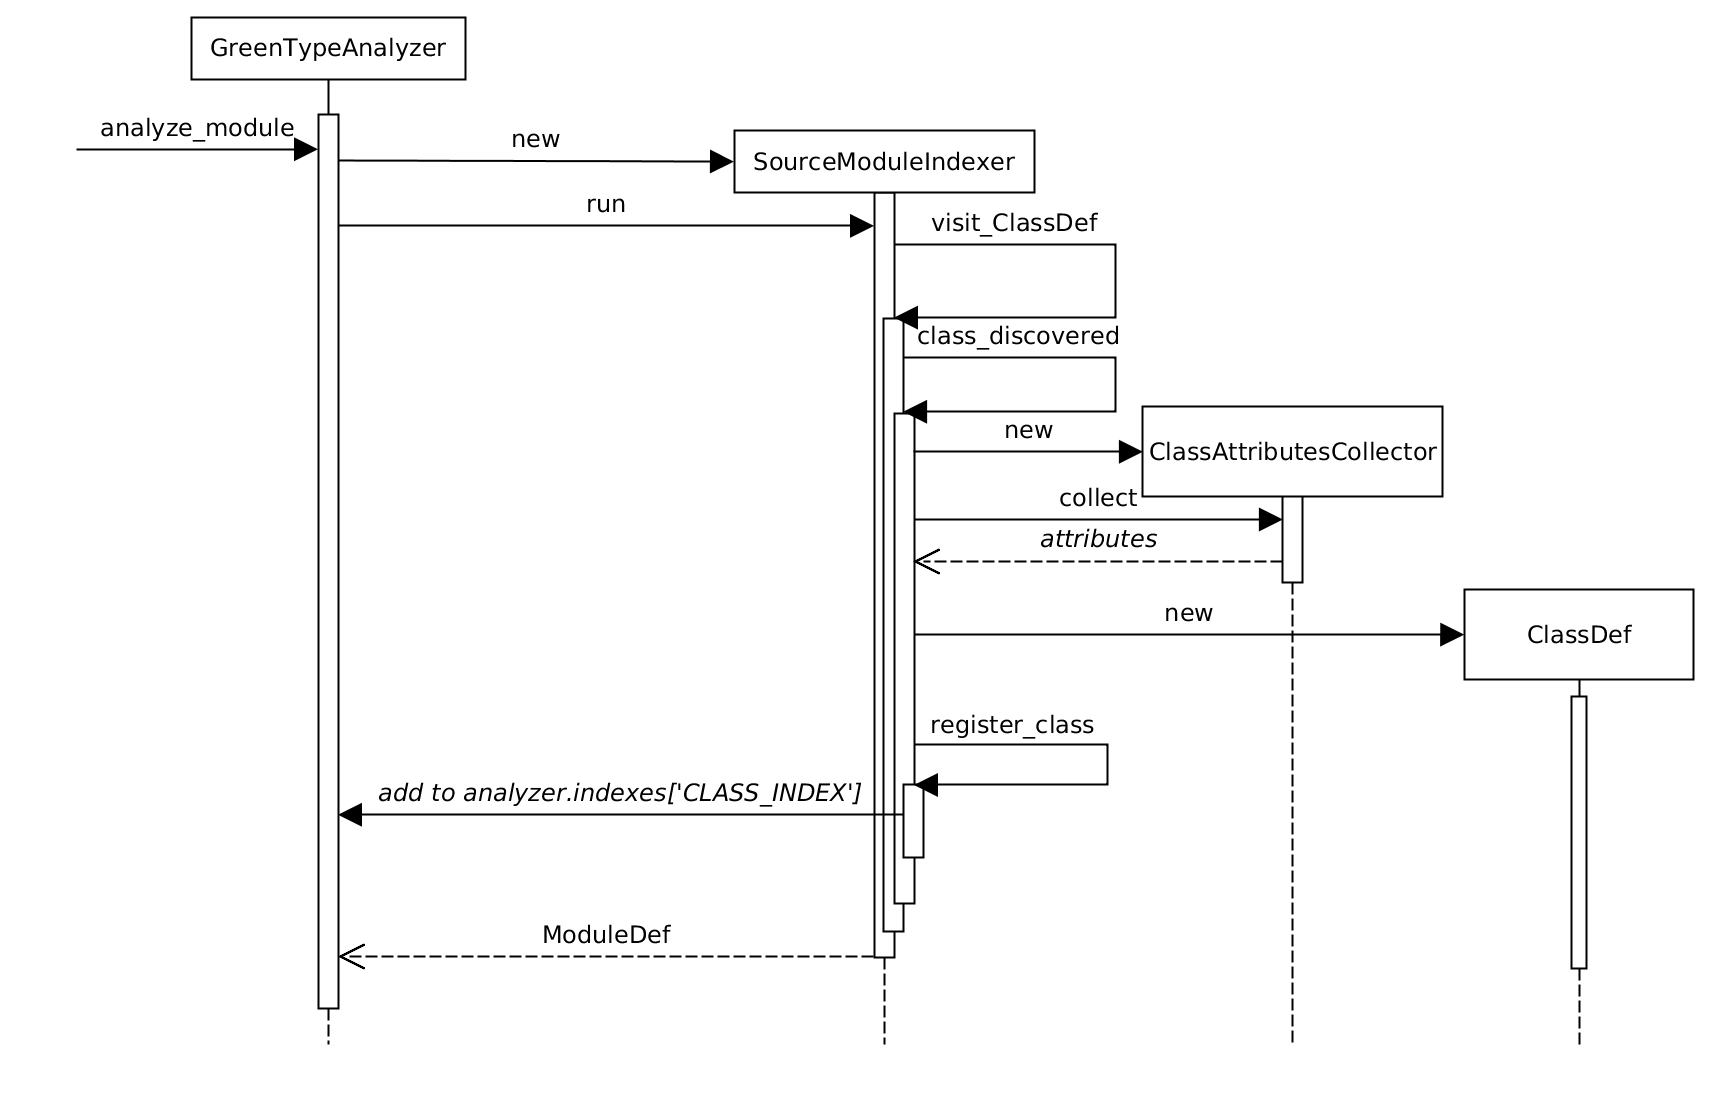
\includegraphics[width=\textwidth]{fig/indexing-diag.png}
  \end{center}
  \caption{Диаграмма процесса индексации модуля}
  \label{fig:indexing-diag}
  \end{figure}

  \item[Config] \hfill \\
    Настройки для анализатора могут быть указаны, как через аргументы командной
    строки (для чего используется стандартный модуль !argparse!), так и через
    конфигурационный файл !greentype.cfg! (на данный момент только пути поиска
    модулей --- !source-roots!) , что было необходимо для анализа
    проектов в режиме сбора статистики (подробнее в разделе
    \ref[sec:statistics-collecting]). Для того чтобы убрать из
    !GreenTypeAnalyzer! логику разбора аргументов и чтения файла конфигурации, а
    также сделать добавление новых настроек проще, его настройки представлены
    экземпляром класса !Config!. Он имеет такой же интерфейс, что и стандартная
    коллекция !dict!, однако также включает вспомогательные методы
    !update_from_object! и !update_from_cfg_file!. Пример файла формата файла
    конфигурации приведен в листинге~\ref{lst:config-file-sample}. Все настройки
    анализатора, их назначение и формат соответствующих аргументов командной
    строки приведены на таблице~ref{tab:config-ref}.
  \item[StatisticsReport] \hfill \\
    Первоначально различная статистика в проекте, например, суммарное количество
    проиндексированных модулей, классов, функций и параметров, количество
    параметров, для которых был найден только один подходящий класс
    (!single_type_parameters!) или количество параметров, для которых нашлось
    несколько классов или вообще ни одного , подсчитывалась и отображалась в
    консоли в неструктурированном виде. Однако это оказалось неудобно для
    последующей оценки полученных данных и подсчета статистики. Поэтому подсчет
    и форматирование результатов статистики были вынесены в отдельный класс
    !StatisticsReport!. Он имеет ряд вспомогательных методов для анализа
    содержимого индексов (например,!undefined_parameters!  или
    !scattered_type_parameters!), а полученные результаты могут быть
    представлены в виде текстового отчета (!format_text!) или JSON
    (!format_json!). 

  
\end{description}

\begin{lstlisting}[
language=,
label=lst:config-file-sample,
caption={Пример формата файла конфигурации}
]
[greentype]

source-roots = devel/src
\end{lstlisting}

\begin{table}[H]
  \small
  \caption{Параметры конфигурации анализатора.}
  \label{tab:config-ref}
  \begin{tabularx}{\textwidth}{ |X|X|X| }
    \hline
    Название & Аргумент командной строки & Значение \\
    \hline
    \texttt{TARGET\_NAME} & \texttt{-t}, \texttt{--target} &  Фильтрация
    объектов, отображаемых в статистике по префиксу квалифицированного имени.
    \\ \hline

    \texttt{VERBOSE} & \texttt{-v}, \texttt{--verbose} & Режим подробного
    (verbose) вывода, включающего сообщения логгирования с уровнем
    \texttt{DEBUG} и выше.
    \\ \hline

    \texttt{FOLLOW\_IMPORTS} & \texttt{-L}, \texttt{--follow-imports} & 
    Индексация импортируемых модулей (обход модулей проекта в DFS порядке).
    \\ \hline

    \texttt{ANALYZE\_BUILTINS} & \texttt{-B}, \texttt{--no-builtins} &
    Рефлексивно анализировать встроенные (скомпилированные) модули стандартной
    библиотеки.
    \\ \hline

    \texttt{BUILTINS} & --- & Список встроенных модулей для рефлексивной
    индексации.
    \\ \hline
    
    \texttt{SOURCE\_ROOTS} & \texttt{--src-roots} & Корневые каталоги проекта.
    Необходимы для поиска модулей по имени.  
    \\ \hline

    \texttt{TARGET\_PATH} & обязательный аргумент & Начальный каталог или
    конкретный модуль, с которого начинается анализ проекта.
    \\ \hline

  \end{tabularx}
\end{table}

\section{Сбор статистики}
\label{sec:statistics-collecting}

Для оценки эффективности предложенного метода вывода типов параметров функций,
прототип собирает статистику по результатам анализа. Измеряемые метрики включают
в себя:

\begin{enumerate}
  \item Количество проиндексированных модулей, классов, функций и параметров в
    проекте (без зависимостей и стандартной библиотеки) и в целом.

  \item Параметры функций, содержащие максимальное число уникальных атрибутов, к
    которым происходило обращение. В отчет также могут быть включены примеры
    параметров с наибольшим числом обращений к атрибутам.

  \item Параметры функций, к атрибутам которых не происходило обращений в теле
    функции (\emph{attributeless parameters}). Для них также
    собирается информация о том, какие из них тем не менее использовались в
    качестве возвращаемого значения функции (!ParameterDef.returned!), операнда
    в арифметическом выражении (!ParameterDef.used_as_operand!) или аргумента
    другой функции (!ParameterDef.used_as_argument!).

  \item Параметры функций, к атрибутам которых происходило обращение, но для
    которых тем не менее не было найдено ни одного подходящего класса
    (\emph{undefined parameters}).

  \item Параметры функций, к атрибутам которых происходило обращение, и для
    которых был найден только один подходящий класс (\emph{exact type parameters}).

  \item Параметры функций, к атрибутам которых происходило обращение, но для
    которых было найдено более одного подходящего класса (\emph{scattered type
      parameters}).

\end{enumerate}

Все группы параметров для чистоты измерений включают только параметры функций
проекта. В результаты измерений также можно включить примеры параметров каждой из
групп. Статистика собранная для ряда публично доступных проектов на Python,
обсуждается в разделе~\ref{sec:projects-analysis}.

